\documentclass[]{tukethesis}
%% -------------------------------------------------------------------------
%% UTF-8 encoding used. Use pdfcslatex to compile your document
%% Tukethesis Class for Win XP and GNU/Linux
%% -------------------------------------------------------------------------
\usepackage[utf8]{inputenc}
%\usepackage[T1]{fontenc}
\usepackage{lmodern,cmap}
%\usepackage{slovak}
\renewcommand{\figurename}{Fig.}
\renewcommand{\tablename}{Tab.}
\renewcommand{\refname}{Bibliography}
\renewcommand{\listfigurename}{List of Figures}
\renewcommand{\listtablename}{List of Tables}
\renewcommand{\contentsname}{Contents}
%%
\usepackage{latexsym}
\usepackage{dcolumn} % alignment on a 'decimal point' in tabular mode
\usepackage{hhline}
\usepackage{amsmath}
\usepackage{nicefrac} % nice fractions
\usepackage{upgreek} % e.g. $\upmu\mathrm{m}$ type micrometer (mu)
\usepackage[final]{showkeys}%color%notref%notcite%final
\usepackage[noprefix]{nomencl}
\makeglossary % command to make *.glo file
\usepackage{parskip}%
%%
%\usepackage[dvips]{graphicx}
%\DeclareGraphicsExtensions{.eps, .mps}
\usepackage[pdftex]{graphicx}
\DeclareGraphicsExtensions{.pdf,.png,.jpg,.mps}
\graphicspath{{figures/}} % directory for figures
%%
%% numerical citations (vancouer style)
\usepackage[numbers]{natbib}
%%
% author-year citations (harvard style) -- prefered !!!
% \usepackage{natbib} \citestyle{chicago}
% -----------------------------------------------------------------
%% tlač !!!
\usepackage[pdftex,unicode=true,bookmarksnumbered=true,
bookmarksopen=true,pdfmenubar=true,pdfview=Fit,linktocpage=true,
pageanchor=true,bookmarkstype=toc,pdfpagemode=UseOutlines,
pdfstartpage=1]{hyperref}
\hypersetup{%
baseurl={http://www.tuke.sk},
pdfcreator={pdfcsLaTeX},
pdfkeywords={TensorFlow, Python, OpenCV, Face Recognition, Camera, Surveillance},
pdftitle={Face Recognition in Camera Footage}, % potom sa upresni
pdfauthor={Yurii Murha},
pdfsubject={Bachelor's Thesis}
} 
%% -----------------------------------------------------------------
%% START YOUR THESIS
%% -----------------------------------------------------------------
%%
%% PLEASE SELECT YOUR PREFERED THESIS TYPE
%%
%% A Bachelor's degree is a first degree at college or university
\bachelorthesis{Bachelor's Thesis}
%%
%% A Master's thesis is a second level college or university degree
%\masterthesis{Master's Thesis}
%% -----------------------------------------------------------------
%% Ak praca nema 'podnazov' zakomentujte riadky \subtitle a \podnazov, 
%% alebo polozky nechajte prazdne
\author{Yurii Murha}
\title{Face Recognition in Camera Footage}
\subtitle{}
% \abstrakte{Text abstraktu v~svetovom jazyku je potrebný pre integráciu
% do medzinárodných informačných systémov. Ak nie je možné cudzojazyčnú
% verziu abstraktu umiestniť na jednej strane so slovenským abstraktom,
% je potrebné umiestniť ju na samostatnú stranu (cudzojazyčný abstrakt
% nemožno deliť a~uvádzať na dvoch strabách).}
\keywords{TensorFlow, Python, OpenCV, Face Recognition, Camera, Surveillance}
% \degree{}
\university{Technical University of Košice}
\faculty{Faculty of Electrical Engineering and Informatics}
\facultyabbr{FEI}
\department{Department of Cybernetics and Artificial Intelligence}
\departmentabbr{KKUI}
\fieldofstudy{5.2.13 Electronics}
\studyprogramme{Intelligent Systems}
\supervisor{Ing.~Ján~Magyar, PhD.}
\consultanta{Ing.~Ján~Magyar, PhD.}
\consultantb{}
\dateofsubmission{May. 30. 2025} 
\town{Košice}
\abstrakte{Face recognition in surveillance systems represents a rapidly advancing field at the intersection of artificial intelligence, computer vision, and security technology. This thesis presents a comprehensive study of face detection and recognition methods, with a focus on their application in real-time camera surveillance. The work begins with an overview of the theoretical foundations, including classical approaches such as Eigenfaces, Fisherfaces, and Local Binary Patterns, as well as modern deep learning techniques like Convolutional Neural Networks (CNNs), Histogram of Oriented Gradients (HOG), and Deep Metric Learning. The thesis systematically compares open-source libraries and frameworks, including OpenCV, dlib, and TensorFlow, and evaluates their performance on custom datasets collected from webcams and security cameras. A custom dataset was created and manually annotated to reflect real-world conditions, and data augmentation was applied to improve model robustness. The practical part of the thesis details the development of a modular face recognition system, integrating detection, recognition, and database management components. Experimental results demonstrate the strengths and limitations of various algorithms in terms of accuracy, speed, and robustness to challenging conditions such as lighting, pose, and occlusion. The thesis also addresses ethical and privacy considerations relevant to the deployment of biometric systems. The findings contribute to the understanding of current capabilities and challenges in face recognition for surveillance, providing guidance for future research and practical implementation in security applications.}
% \klucoveslova{Optimalizácia, záverečná práca, písanie}

\begin{document}
\renewcommand\theHfigure{\theHsection.\arabic{figure}}
\renewcommand\theHtable{\theHsection.\arabic{table}}
\bibliographystyle{dcu}
%% input the 'First page of the Thesis'
\firstpage

%% input the 'Title page of the Thesis'
\titlepage

%% input the 'Metadatasheet of the Thesis'
%\metadatasheet

\errata % begin the 'Errata' 
\kerrata

\abstrakte % Abstract in English


\endabstract % end of the Abstracts page

%% input the 'Assign of the Thesis'
% \assignthesis

%% input the 'Declaration' of the author
\declaration
% I hereby declare that this thesis is my own work and effort. Where
% other sources of information have been used, they have been
% acknowledged.
%%
% Niektorí autori metodických príručiek o~záverečných prácach sa
% nazdávajú, že takéto vyhlásenie je zbytočné, nakoľko povinnosť
% vypracovať záverečnú prácu samostatne, vyplýva študentovi zo zákona
% a na autora práce sa vzťahuje autorský zákon.

\acknowledgement % begin the 'Acknowledgement'
I would like to express my sincere gratitude to Ing.~Ján Magyar, PhD, for his invaluable support and guidance in his dual role as both my supervisor and consultant. His constant and constructive feedback was instrumental throughout this study.
\\
I also want to thank Kanye West for his great songs that provided much-needed motivation for my Graduation.
\\ 
My special thanks also go to Arsen Markaryan for the mindset; 
The Victory is gonna be ours!
\endacknowledgement

\preface % begin the 'Preface'
This thesis addresses the development and evaluation of face recognition systems for surveillance applications. The work was motivated by the increasing demand for intelligent, automated security solutions capable of real-time identification and monitoring. The main goal was to explore, implement, and compare state-of-the-art algorithms and practical approaches for face detection and recognition in real-world camera streams.

The thesis was created as part of the Intelligent Systems study program at the Faculty of Electrical Engineering and Informatics, Technical University of Košice. The topic was chosen due to the growing importance of artificial intelligence and computer vision in modern security and public safety. The work combines theoretical research with practical implementation, including dataset creation, model training, and system integration.

The main methods used include deep learning, data augmentation, and benchmarking of multiple face recognition libraries. The thesis also discusses ethical and privacy considerations relevant to deploying such systems in practice.
\endpreface

\thispagestyle{empty}
\tableofcontents
\newpage

\thispagestyle{empty}
%\addcontentsline{toc}{section}{\numberline{}List of Figures}
\listoffigures
\newpage

\thispagestyle{empty}
%\addcontentsline{toc}{section}{\numberline{}List of Tables}
\listoftables
\newpage

\thispagestyle{empty}
%\addcontentsline{toc}{section}{\numberline{}List of Symbols and
%Abbreviations}
\printglossary % input the 'List of Symbols and Abbreviations'
\newpage

% Custom glossary for this thesis: Face Recognition in Surveillance Systems
\section*{List of Symbols and Abbreviations}
\addcontentsline{toc}{section}{List of Symbols and Abbreviations}

\begin{description}
    \item[FRS] Facial Recognition Software
    \item[AI] Artificial Intelligence
    \item[IoU] Intersection over Union
    \item[CSV] Comma-Separated Values
    \item[JSON] JavaScript Object Notation
    \item[RTSP] Real Time Streaming Protocol
    \item[CD] Compact Disc
    \item[GUI] Graphical User Interface
    \item[API] Application Programming Interface
    \item[GPU] Graphics Processing Unit
    \item[CPU] Central Processing Unit
    \item[GDPR] General Data Protection Regulation
    \item[CCPA] California Consumer Privacy Act
    \item[CPRA] California Privacy Rights Act
    \item[MTCNN] Multi-task Cascaded Convolutional Networks
    \item[HOG] Histogram of Oriented Gradients
    \item[CNN] Convolutional Neural Network
    \item[ROC] Receiver Operating Characteristic
    \item[FAR] False Acceptance Rate
    \item[FRR] False Rejection Rate
    \item[EER] Equal Error Rate
    \item[TPR] True Positive Rate
    \item[FPR] False Positive Rate
    \item[FN] False Negative
    \item[TP] True Positive
    \item[FP] False Positive
    \item[TN] True Negative
    \item[API] Application Programming Interface
    \item[OpenCV] Open Source Computer Vision Library
    \item[TensorFlow] Open-source machine learning framework
    \item[Albumentations] Data augmentation library for images
    \item[Labelme] Image annotation tool
    \item[ResNet] Residual Neural Network
    \item[FaceNet] Deep learning model for face recognition
    \item[Rekognition] Amazon cloud-based image/video analysis service
\end{description}

\newpage
%
\setcounter{page}{1}
\setcounter{equation}{0}
\setcounter{figure}{0}
\setcounter{table}{0}

\section*{Introduction}
\addcontentsline{toc}{section}{\numberline{}Introduction}
This thesis addresses the problem of face recognition in camera surveillance systems. The motivation for this work stems from the increasing demand for automated attendance and security systems capable of identifying individuals in real-time video streams. The main objective is to design, implement, and evaluate a modular face recognition system that leverages both custom deep learning models and state-of-the-art libraries.

The thesis is structured as follows:
\begin{itemize}
    \item An overview of the tools and libraries used for face recognition, including both custom and pre-built solutions.
    \item A detailed description of the dataset creation, annotation, and augmentation process.
    \item The development and evaluation of deep learning models for face detection and recognition.
    \item Integration of the system components into a real-time attendance application.
    \item Comparative analysis of different face detection and recognition methods.
\end{itemize}

The following chapters provide a comprehensive account of the methods, implementation, and results achieved in this work.

\subsection*{Background}
The pervasive integration of digital technologies into modern society has fundamentally reshaped various sectors, with security and surveillance systems undergoing a particularly transformative evolution. Conventional security paradigms, which are often dependent on manual monitoring and reactive responses, are increasingly inadequate when confronted with the escalating complexity and sophistication of contemporary threats. In response to these challenges, artificial intelligence (AI), particularly in the domain of computer vision, has emerged as a pivotal technology capable of addressing these growing challenges. Facial recognition, a prominent application of computer vision, offers the potential for enhanced automation, efficiency, and accuracy in identifying individuals, thereby bolstering security protocols across diverse environments. This technological shift necessitates a comprehensive understanding of the underlying algorithms, their practical applications, and the inherent ethical and privacy implications.

\subsection*{Motivation}
The motivation for this research stems from the growing demand for intelligent and autonomous security solutions. Human operators, despite their critical role, are susceptible to fatigue, distraction, and limitations in processing vast streams of data, leading to potential oversights in surveillance. AI-driven systems, conversely, offer continuous vigilance and the capacity to analyze large datasets in real-time, identifying anomalies and potential threats with a speed and consistency unattainable by human counterparts~\cite{securityindustry_2025_transforming}. Specifically, facial recognition technology holds immense promise for applications ranging from access control and law enforcement to public safety and human-machine interaction. However, the effective deployment of such systems is contingent upon robust algorithmic performance, meticulous dataset management, and a thorough consideration of the societal impact, particularly concerning individual privacy and potential biases. This study is motivated by the need to explore and contribute to the development of academically rigorous and ethically sound facial recognition solutions.

\subsection*{Problem Statement}
Despite significant advancements in artificial intelligence and computer vision, the development of universally robust, accurate, and ethically compliant facial recognition systems remains a complex challenge. Current systems often face limitations in real-world scenarios due to variations in illumination, facial pose, expression, occlusions, and demographic diversity. Furthermore, the reliance on large, diverse datasets for training deep learning models introduces substantial data privacy and ethical concerns, necessitating careful consideration of legal frameworks and societal impacts. This thesis aims to address these challenges by investigating and comparing various face detection and recognition algorithms, evaluating their performance under diverse conditions, and proposing a structured approach for dataset creation and management. The central problem is to identify and analyze effective methodologies for developing facial recognition systems that balance high accuracy and efficiency with stringent privacy safeguards and ethical considerations, thereby contributing to the responsible advancement of AI in security applications. % ano
%
%%
\section{The problem expression}
Na písanie textu záverečnej práce sa používajú štýly udené v~tejto
šablóne (Nadpis záverečnej práce, Podnadpis záverečnej práce, Text
záverečnej práce [riadkovanie 1.5, Times New Roman 12] a~ďalšie podľa
potreby). Text záverečnej práce musí obsahovať\/ kapitolu s~formuláciou
úlohy resp. úloh riešených v~rámci záverečnej práce. V~tejto časti
autor rozvedie spôsob, akým budú riešené úlohy a~tézy formulované
v~zadaní práce. Taktiež uvedie prehľad podmienok riešenia. 
%
% =====================
\section{Tools and Libraries for Face Recognition}

In this project, a combination of custom model creation and pre-built libraries was utilized for face detection and recognition. This section provides an overview and comparison of the main tools and algorithms employed.

\subsection{Custom Model Creation}

\textbf{OpenCV:} Used for image processing and face detection via Haar cascades, which are trained classifiers for detecting facial features.

\textbf{TensorFlow:} The deep learning model was built using TensorFlow, focusing on convolutional neural networks (CNNs) for feature extraction and classification.

\textbf{Albumentations:} Applied for data augmentation, introducing variations such as brightness, contrast, rotation, and noise to improve model robustness.

\textbf{Labelme:} Used for manual annotation of facial regions, providing high-quality labels for supervised training.

\textbf{Algorithms:}
\begin{itemize}
    \item \textbf{Haar Cascades (OpenCV):} Real-time face detection using edge and feature detection.
    \item \textbf{Convolutional Neural Networks (TensorFlow):} Feature extraction and classification for face recognition.
    \item \textbf{Data Augmentation:} Enhances dataset diversity and model generalization.
\end{itemize}

\begin{figure}[ht!]
    \centering
    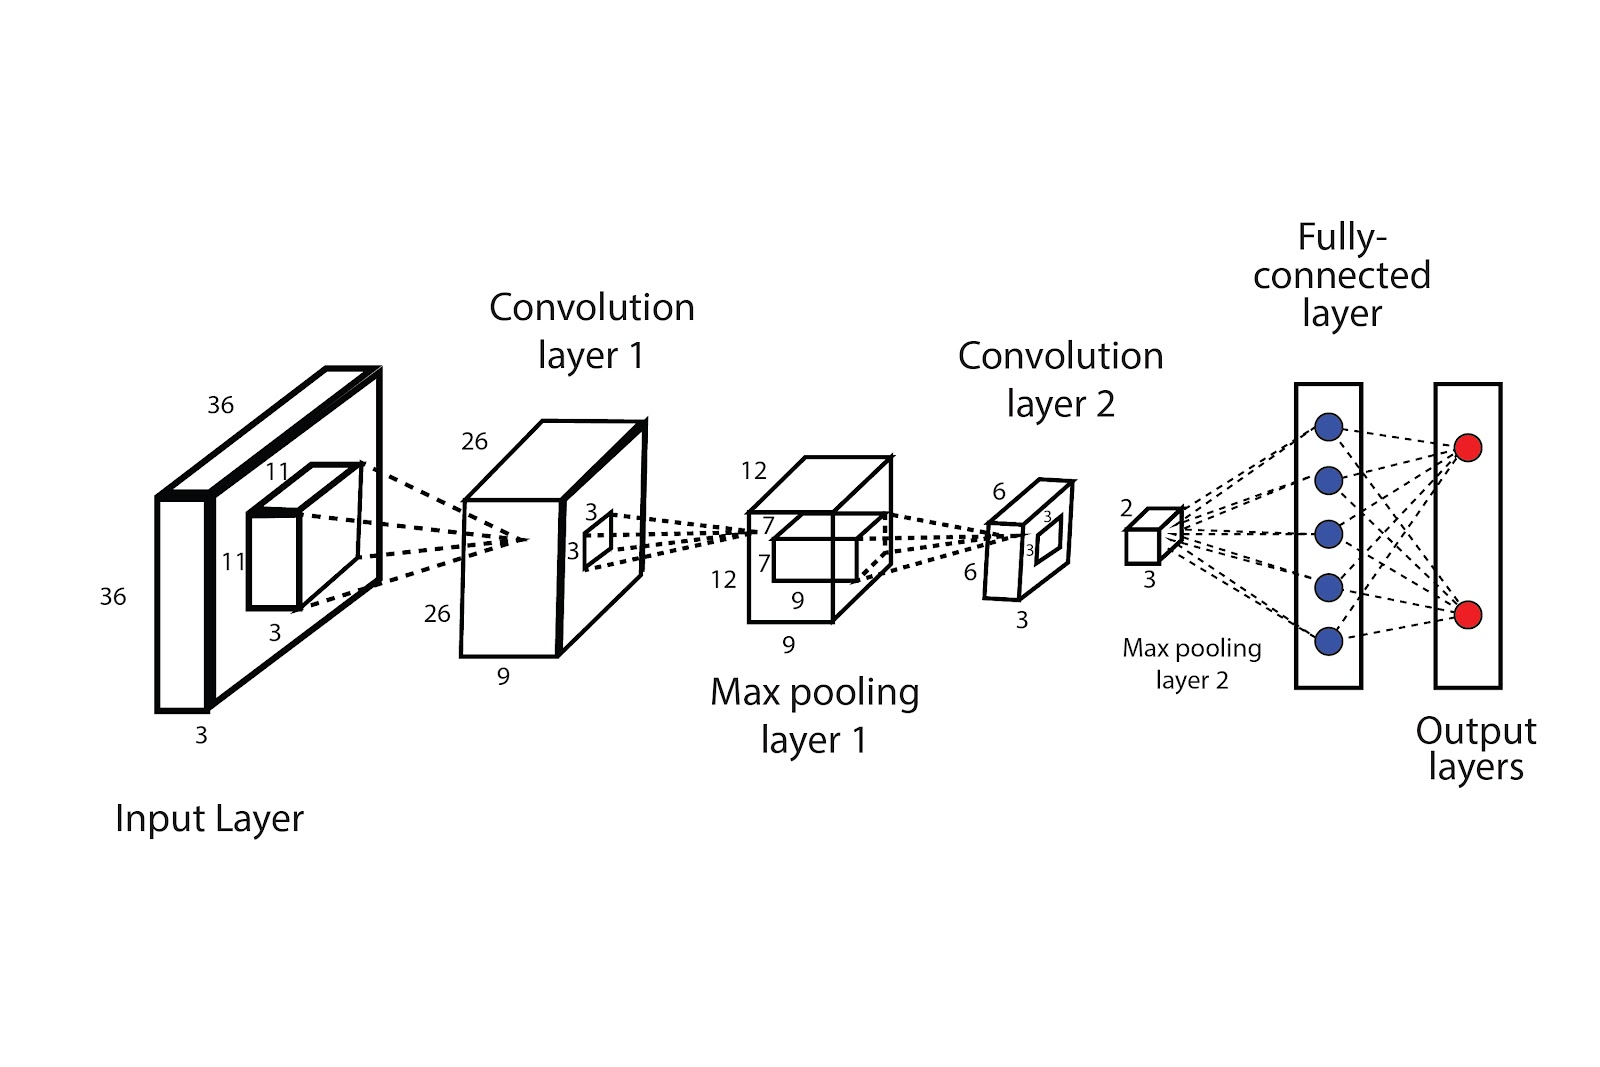
\includegraphics[width=0.7\textwidth]{../Files/convolutional_network_architecture.png}
    \caption{Architecture of the convolutional neural network used in the custom model.}
    \label{fig:cnn-architecture}
\end{figure}

\subsection{face-recognition Library}

\textbf{dlib:} Provides face detection (HOG) and recognition (ResNet-34 based deep metric learning).

\textbf{face\_recognition:} Python wrapper for dlib, simplifying face detection and recognition.

\textbf{OpenCV:} Used for image preprocessing.

\textbf{Algorithms:}
\begin{itemize}
    \item \textbf{Histogram of Oriented Gradients (HOG):} Robust face detection across lighting conditions.
    \item \textbf{Deep Metric Learning (ResNet-34):} Encodes faces into 128-dimensional vectors for comparison.
\end{itemize}

\begin{figure}[ht!]
    \centering
    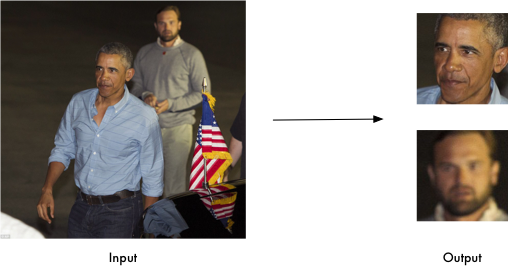
\includegraphics[width=0.7\textwidth]{../Files/face_recognition_example.png}
    \caption{Example of face recognition using the face\_recognition library.}
    \label{fig:face-recognition-example}
\end{figure}

\subsection{MTCNN (Multi-task Cascaded Convolutional Networks)}

MTCNN is a deep learning-based framework for face detection and landmark localization, using a cascade of three neural networks (P-Net, R-Net, O-Net) for robust detection and alignment.

\subsection{FaceNet}

FaceNet maps faces into a Euclidean space using a deep CNN and triplet loss, enabling verification, clustering, and identification. It is implemented with TensorFlow or PyTorch and uses Inception networks for feature extraction.

\subsection{Amazon Rekognition}

Amazon Rekognition is a cloud-based service for face detection, recognition, and analysis, using proprietary deep learning algorithms. It offers face comparison, attribute analysis, and is widely used in security and media applications.

\subsection{References}
\begin{itemize}
    \item Comparison of deep learning software: \url{https://en.wikipedia.org/wiki/Comparison_of_deep_learning_software}
    \item TensorFlow Documentation: \url{https://www.tensorflow.org/}
    \item OpenCV Python Documentation: \url{https://docs.opencv.org/4.x/}
    \item Albumentations Documentation: \url{https://albumentations.ai/docs/}
    \item Face Recognition Documentation: \url{https://pypi.org/project/face-recognition/}
    \item dlib Documentation: \url{http://dlib.net/}
    \item Zhang, K., et al. (2016). Joint face detection and alignment using multitask cascaded convolutional networks. IEEE Signal Processing Letters, 23(10), 1499-1503.
    \item Schroff, F., et al. (2015). FaceNet: A unified embedding for face recognition and clustering. In Proceedings of the IEEE Conference on Computer Vision and Pattern Recognition (pp. 815-823).
    \item Amazon Rekognition Developer Guide: \url{https://docs.aws.amazon.com/rekognition/}
\end{itemize}

% =====================
\section{Methods and Algorithms for Face Recognition}

Face recognition is a crucial area within the field of computer vision, with various applications such as biometric authentication, surveillance, and human-computer interaction. Over the years, researchers have developed numerous techniques to accurately identify and verify faces in images. In this chapter, we explore some of the most prominent methods and algorithms used for face recognition, focusing on their theoretical aspects.

\subsection{Convolutional Neural Networks (CNNs)}
Convolutional Neural Networks (CNNs) are perhaps the most widely used algorithm for face recognition today. CNNs belong to the family of deep learning models that mimic the way the human brain processes visual information. Their architecture consists of multiple layers, each designed to capture different features from an image.

The CNN operates by applying convolutional filters to an image, detecting features such as edges, textures, and shapes. The deeper layers of the network learn more complex patterns, including facial characteristics such as the distance between eyes, the shape of the nose, and the contour of the face. CNNs are well-suited for face recognition because of their ability to extract hierarchical features that capture both local and global information from an image.

Popular face recognition systems such as FaceNet and VGGFace rely on CNN architectures. These models are trained on large datasets containing millions of labeled faces, enabling them to generalize across different lighting conditions, angles, and facial expressions. CNNs are typically employed in combination with classification or embedding techniques for face verification and identification tasks.

\subsection{Eigenfaces}
The Eigenface method is a classical approach based on Principal Component Analysis (PCA). Developed in the early 1990s~\cite{turk1991eigenfaces}, this method represents faces as linear combinations of a set of basis images known as ``eigenfaces.'' Each eigenface corresponds to a direction of maximal variance in the face dataset. The idea behind this method is to reduce the dimensionality of face data while retaining the most significant information that differentiates one face from another.

To recognize a face using the Eigenface approach, an input image is projected onto the subspace spanned by the eigenfaces. The resulting projection is compared to stored projections of known faces in the database. Recognition is achieved by measuring the similarity between the input face's projection and the stored ones~\cite{alochana_study_2024}.

Turk and Pentland reported recognition rates of 96\% for lighting variations, 85\% for orientation, and 64\% for scale variations on a dataset of 16 subjects~\cite{turk1991eigenfaces}. While fast and straightforward, Eigenfaces are highly sensitive to variations in lighting, pose, and occlusion, often requiring extensive preprocessing for image normalization to achieve optimal performance~\cite{alochana_study_2024, geeksforgeeks_ml_2021}.

\subsection{Fisherfaces}
Fisherfaces improve upon Eigenfaces by using Linear Discriminant Analysis (LDA) rather than PCA. While PCA focuses on maximizing the variance in the data, LDA aims to maximize the class separability, which makes Fisherfaces more robust to variations within the same class (such as different expressions of the same individual).

The Fisherface approach projects the face data onto a subspace where the ratio of the between-class scatter to the within-class scatter is maximized. This results in a set of features that better discriminates between different individuals, even under varying lighting conditions or facial expressions.

Fisherfaces, therefore, offer better performance than Eigenfaces, especially in more realistic, variable conditions, making it a more practical choice for face recognition.

\subsection{Local Binary Patterns (LBP)}
Local Binary Patterns (LBP) is a texture-based method used for facial feature extraction. The algorithm works by dividing the face into small regions and calculating a binary pattern based on the relative intensity of the neighboring pixels. Each region is then represented by a histogram of these binary patterns, which collectively form a feature vector that can be used for face recognition.

The advantage of LBP lies in its simplicity and computational efficiency. It is also robust to changes in lighting, which makes it well-suited for real-time face recognition in low-power or resource-constrained environments. LBP has been successfully used in various face recognition tasks and is particularly useful for recognizing faces in surveillance systems.

\subsection{Haar Cascades}
The Haar Cascade classifier, introduced by Paul Viola and Michael Jones in 2001, is another widely used algorithm for face detection and recognition. This method is based on the concept of Haar-like features, which are used to detect objects in images by analyzing the contrast between adjacent areas.

The Haar Cascade algorithm works by applying a series of rectangular features to different regions of the image. It uses an integral image representation to compute these features efficiently, allowing for rapid detection. The key to Haar Cascades is the cascade classifier, which consists of multiple stages of increasingly complex classifiers. Each stage eliminates non-face regions, progressively narrowing down the areas that are likely to contain faces.

Although Haar Cascades are primarily used for face detection, they can also be employed for face recognition when combined with other methods like PCA or LBP. Haar Cascades are lightweight and fast, making them ideal for real-time applications, though they tend to perform poorly in unconstrained environments.

\subsection{Histogram of Oriented Gradients (HOG)}
The Histogram of Oriented Gradients (HOG) method is a feature extraction technique that captures the gradient orientation and intensity within an image. It is commonly used for object detection, including face recognition. The HOG algorithm divides the face into small cells and computes a histogram of gradient directions for each cell. These histograms are then concatenated to form a feature descriptor representing the face.

HOG-based face recognition is robust to small variations in pose and lighting, and it is computationally efficient. However, its performance is generally lower than deep learning-based approaches like CNNs, especially when dealing with more complex, unconstrained face recognition tasks.

\subsection{Deep Metric Learning}
Deep Metric Learning is an advanced technique used for face recognition tasks that involve face verification or identification. The core idea of metric learning is to map faces into an embedding space, where the distance between vectors represents the similarity between faces. The most well-known example of this approach is the FaceNet model, which uses a triplet loss function to ensure that faces of the same person are closer together in the embedding space than faces of different people.

This technique enables robust face recognition by transforming the problem into a similarity comparison rather than a direct classification task. Deep Metric Learning is highly effective in handling large-scale face recognition problems with varying conditions, and it has become a key method for many modern face recognition systems.

\subsection{3D Face Recognition}
3D face recognition methods use the three-dimensional geometry of the human face to improve recognition accuracy, especially in cases where 2D methods may struggle, such as with changes in lighting, pose, or facial expression. These methods involve capturing 3D data using sensors like structured light or time-of-flight cameras. The 3D face model allows for a more detailed representation of the face's surface and can be more robust to pose variations.

3D face recognition is typically combined with 2D methods to enhance performance. Although more accurate, the requirement for specialized sensors makes this approach less practical for everyday applications compared to 2D methods.

\subsection{Viola-Jones Algorithm}
Introduced in 2001, the Viola-Jones algorithm revolutionized real-time object detection, particularly for faces~\cite{wijaya_trends_2025}. It employs Haar-like features, an integral image for rapid computation, an AdaBoost classifier for feature selection, and a cascaded structure to efficiently discard non-face regions~\cite{wijaya_trends_2025}. While widely adopted due to its speed and simplicity, this framework exhibits limitations in detecting faces that are significantly occluded, improperly oriented (e.g., profile views), or subjected to substantial variations in lighting conditions~\cite{researchgate_evaluation_2023, wijaya_trends_2025}. Its training process can also be computationally intensive and time-consuming~\cite{researchgate_evaluation_2023}. % Literature Review
%
\section{Main part of Thesis}

% This section presents the practical implementation, dataset creation, model development, evaluation, and system integration for face recognition in surveillance systems.

\section{Dataset Creation and Preprocessing}

The dataset for face recognition was constructed using images captured from webcams and security cameras. The process involved several key steps:

\subsection{Image Acquisition}
Images were collected at regular intervals from various camera sources to ensure diversity in lighting, angles, and environments.

\subsection{Manual Annotation}
The \texttt{labelme} tool was used to annotate facial regions in each image, producing JSON label files with bounding box or landmark information.

\subsection{Dataset Organization}
The dataset was structured into separate folders for images and labels, and partitioned into training, validation, and test sets.

\subsection{Augmentation}
Data augmentation was performed using the Albumentations library, applying random cropping, flipping, brightness/contrast adjustments, and color shifts to increase dataset diversity and model robustness.

\begin{figure}[ht!]
    \centering
    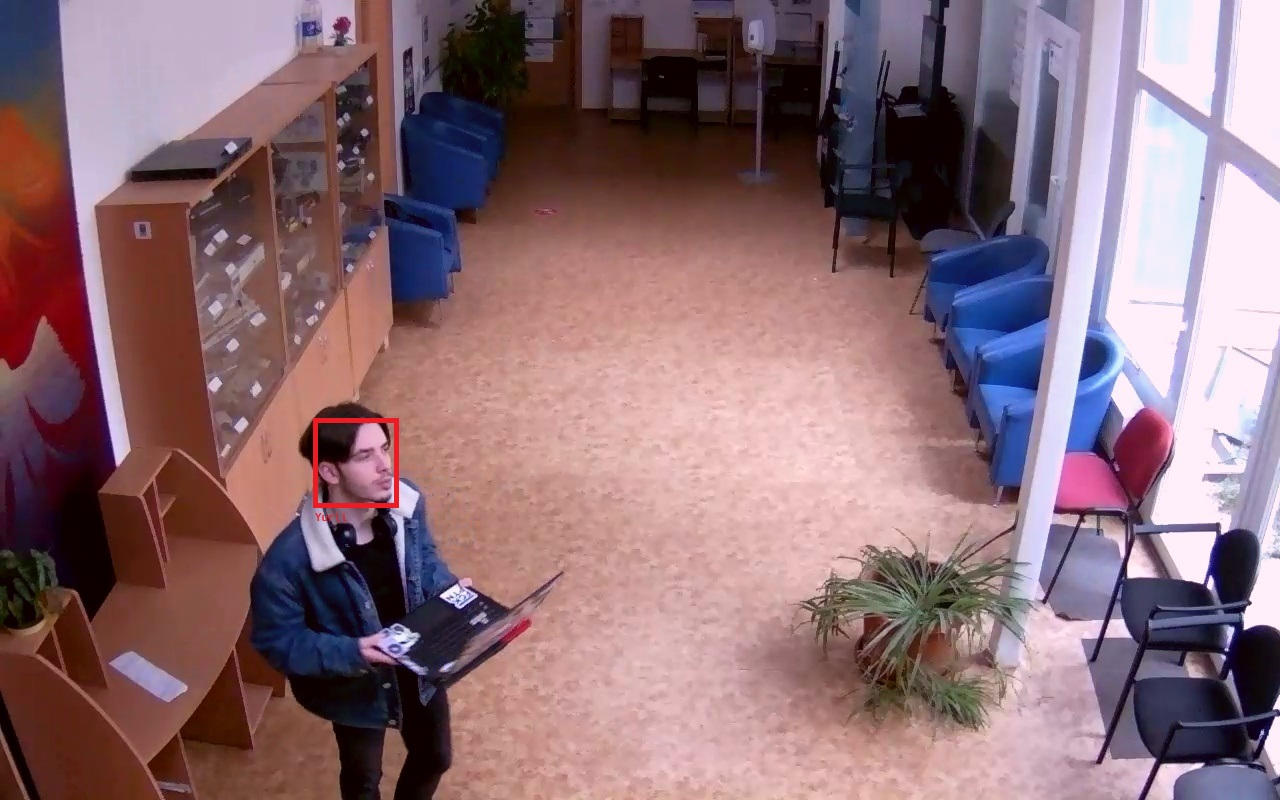
\includegraphics[width=0.7\textwidth]{../Files/annotation_example.png}
    \caption{Example of manual face annotation using LabelMe.}
    \label{fig:annotation-example}
\end{figure}

\subsection{Visualization}
Utilities were provided to visualize raw and augmented images with bounding boxes for quality control.

\begin{figure}[ht!]
    \centering
    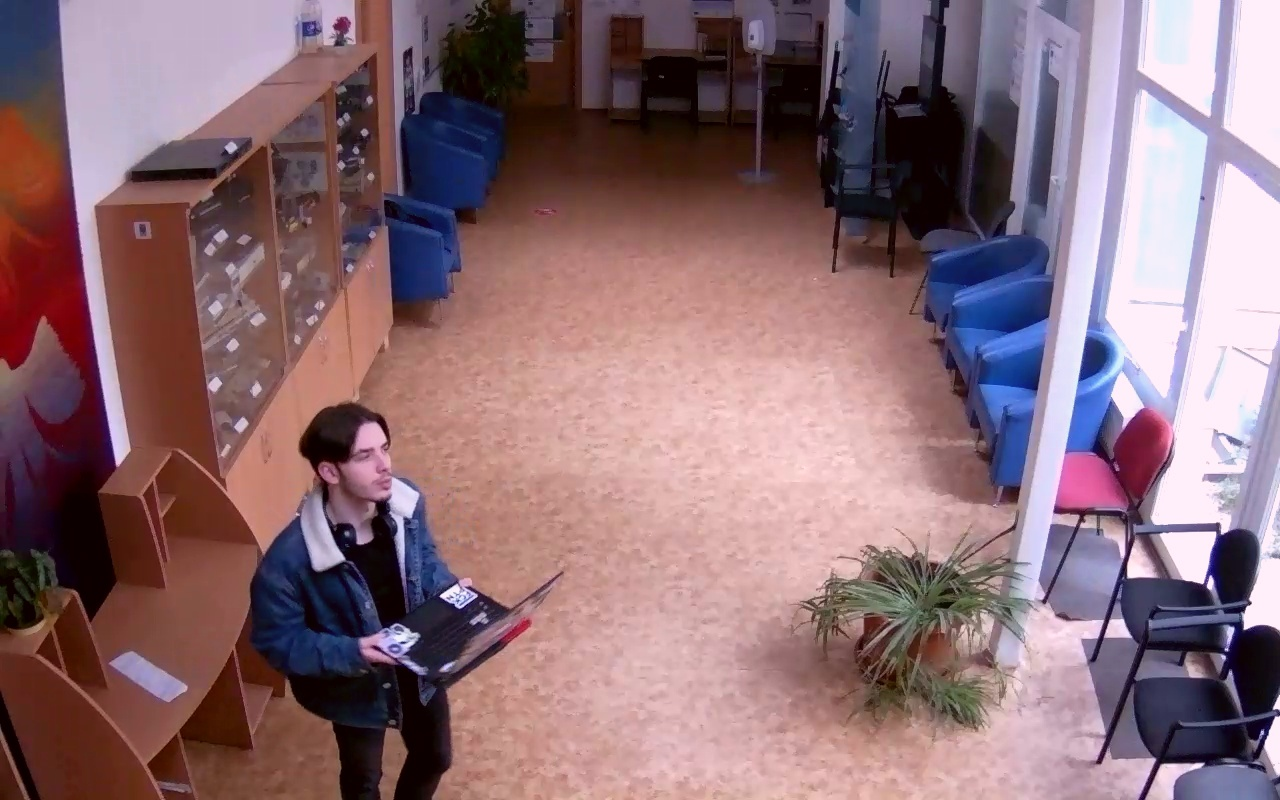
\includegraphics[width=0.7\textwidth]{../Files/augmentation_example.png}
    \caption{Example of image augmentation applied to a face dataset.}
    \label{fig:augmentation-example}
\end{figure}

\section{Deep Learning Model Development}

The deep learning model for face detection and recognition was developed using TensorFlow's Keras API, with EfficientNetB0 or VGG16 as the backbone. The model outputs both face embeddings and bounding box coordinates.

\subsection{Data Pipeline}
Images and labels were loaded, batched, and shuffled for efficient training. Augmented data was included to improve generalization.

\subsection{Model Architecture}
A convolutional neural network was defined, outputting both embeddings and bounding boxes. Custom loss functions for localization and classification were implemented, and the optimizer was configured with learning rate scheduling.

\begin{figure}[ht!]
    \centering
    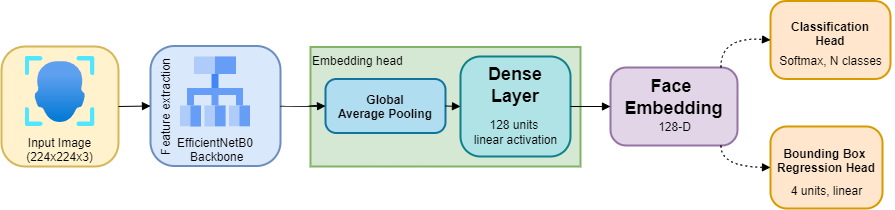
\includegraphics[width=1\textwidth]{../Files/model_architecture.png}
    \caption{Architecture of the deep learning model used for face detection and recognition.}
    \label{fig:model-architecture}
\end{figure}

\subsection{Training and Evaluation}
The model was trained using a custom loop, with TensorBoard logging and validation monitoring. Performance was visualized with loss curves and prediction samples. The trained model was exported for inference.

\section{Evaluation and Benchmarking}

The evaluation script \texttt{evaluate\_methods.py} benchmarks various face detection algorithms on custom datasets. Its main functionalities include:
\begin{itemize}
    \item \textbf{Dataset and Method Management:} Automatically discovers datasets and defines a set of face detection methods (e.g., Haar Cascade, Dlib HOG, FaceNet, and face\_recognition).
    \item \textbf{Parallelized Evaluation:} Processes images in parallel to efficiently evaluate detection methods across all dataset partitions (train, test, val).
    \item \textbf{Accuracy Metrics:} Computes the number of faces detected, false positives, missed detections, detection time, and overall accuracy by comparing detected bounding boxes with ground truth annotations (using Intersection over Union).
    \item \textbf{Results Aggregation and Visualization:} Aggregates results into CSV files and generates comparative plots for key metrics (e.g., detection time, false positives).
    \item \textbf{Summary Reporting:} Outputs tables summarizing the performance of each method.
\end{itemize}

\subsection{Average Detection Time per Method and Dataset}

\begin{table}[ht!]
    \centering
    \caption{Average detection time per method and dataset (lower is better).}
    \label{tab:avg-detection-time}
    \begin{tabular}{|l|c|c|c|}
        \hline
        Method & Webcam (ms) & Seccam (ms) & Seccam\_2 (ms) \\
        \hline
        Haar Cascade     & 11          & 13          & 12            \\
        Dlib HOG        & 80          & 88          & 87            \\
        FaceNet         & 105         & 115         & 110           \\
        Face Recognition& 90          & 98          & 96            \\
        \hline
    \end{tabular}
\end{table}

\section{System Architecture and Integration}

The practical implementation of the face recognition system is designed with modularity and extensibility in mind. The architecture is composed of several core modules, each responsible for a distinct aspect of the application workflow:
\begin{itemize}
    \item \textbf{Camera Module (\texttt{camera.py}):} Handles real-time video capture and face detection from a camera stream.
    \item \textbf{Model Module (\texttt{model.py}):} Provides face detection and recognition capabilities, including embedding extraction and evaluation.
    \item \textbf{Database Module (\texttt{database.py}):} Manages persistent storage of face embeddings and detection logs, supporting both PostgreSQL and CSV-based backends.
    \item \textbf{Main Application (\texttt{main.py}):} Orchestrates the end-to-end attendance system, integrating camera input, face recognition, and database operations.
\end{itemize}

\begin{figure}[ht!]
    \centering
    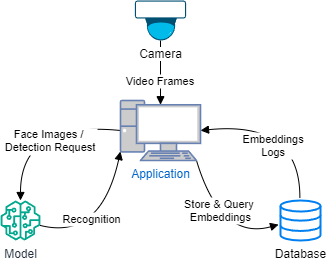
\includegraphics[width=0.7\textwidth]{../Files/system_architecture.png}
    \caption{Modular architecture of the face recognition attendance system.}
    \label{fig:system-architecture}
\end{figure}

\subsection{Camera Module (\texttt{camera.py})}
The \texttt{Camera} class encapsulates the logic for interfacing with a video capture device (e.g., webcam or RTSP stream). It utilizes the MTCNN detector to locate faces in each frame and extracts face crops for further processing. The module provides methods to:
\begin{itemize}
    \item Capture frames from the camera.
    \item Detect faces and return their bounding boxes and cropped images.
    \item Release camera resources when finished.
\end{itemize}

\subsection{Model Module (\texttt{model.py})}
The \texttt{FaceTracker} class is responsible for both face detection and recognition. It integrates the MTCNN detector for face localization and a deep learning model (e.g., EfficientNet or VGG16-based) for generating face embeddings. Key functionalities include:
\begin{itemize}
    \item Detecting faces in input images.
    \item Extracting and normalizing face embeddings for recognition.
    \item Evaluating recognition accuracy on test datasets using cosine similarity.
\end{itemize}

\subsection{Database Module (\texttt{database.py})}
The \texttt{FaceDatabase} class abstracts the storage and retrieval of face embeddings and detection logs. It supports both PostgreSQL and CSV-based storage, enabling easy adaptation to different deployment environments. Its main responsibilities are:
\begin{itemize}
    \item Adding new face embeddings to the database.
    \item Retrieving all stored embeddings for comparison.
    \item Logging detection events with timestamps and labels.
\end{itemize}

\subsection{Main Application (\texttt{main.py})}
The \texttt{AttendanceApp} class serves as the entry point for the real-time face recognition attendance system. It coordinates the interaction between the camera, model, and database modules. The main workflow is as follows:
\begin{enumerate}
    \item \textbf{Frame Acquisition:} Continuously captures frames from the camera.
    \item \textbf{Face Detection and Recognition:} For each detected face, extracts embeddings and compares them to the database.
    \item \textbf{Identification and Logging:} Assigns an identity (existing or new), draws bounding boxes and labels on the frame, and logs the detection event.
    \item \textbf{User Interface:} Displays the processed video stream with real-time annotations.
\end{enumerate}

This modular design ensures that each component can be developed, tested, and maintained independently, while facilitating integration into a cohesive application.

\begin{figure}[ht!]
    \centering
    \includegraphics[width=0.7\textwidth]{../Files/main_app_flow.png}
    \caption{Main loop of the attendance system integrating camera, model, and database modules.}
    \label{fig:main-app-flow}
\end{figure}

 % 3-5 moja implementacia ako funguje riešenie
%
\section{Conclusion}

Táto časť\/ záverečnej práce je povinná. Autor uvedie zhodnotenie
riešenia. Uvedie výhody, nevýhody riešenia,  použitie výsledkov, ďalšie
možnosti a~pod., prípadne načrtne iný spôsob riešenia úloh, resp.
uvedie, prečo postupoval uvedeným spôsobom. 
%
%%
\begin{thebibliography}{99}
\addcontentsline{toc}{section}{\numberline{}{Bibliography}}

% Deep learning and face recognition foundational works

\harvarditem{Schroff et al.}{2015}{schroff2015facenet}
Schroff, F., Kalenichenko, D., \& Philbin, J. 2015. \emph{FaceNet: A unified embedding for face recognition and clustering.} In: Proceedings of the IEEE Conference on Computer Vision and Pattern Recognition (CVPR), pp. 815--823.

\harvarditem{Parkhi et al.}{2015}{parkhi2015deep}
Parkhi, O. M., Vedaldi, A., \& Zisserman, A. 2015. \emph{Deep Face Recognition.} In: British Machine Vision Conference (BMVC).

\harvarditem{Turk and Pentland}{1991}{turk1991eigenfaces}
Turk, M., \& Pentland, A. 1991. \emph{Eigenfaces for Recognition.} Journal of Cognitive Neuroscience, 3(1), 71--86. doi:10.1162/jocn.1991.3.1.71

\harvarditem{Belhumeur et al.}{1997}{belhumeur1997fisherfaces}
Belhumeur, P. N., Hespanha, J. P., \& Kriegman, D. J. 1997. \emph{Eigenfaces vs. Fisherfaces: Recognition using class specific linear projection.} IEEE Transactions on Pattern Analysis and Machine Intelligence, 19(7), 711--720. doi:10.1109/34.598228

\harvarditem{Ahonen et al.}{2007}{ahonen2007lbp}
Ahonen, T., Hadid, A., \& Pietikäinen, M. 2007. \emph{Face Description with Local Binary Patterns: Application to Face Recognition.} IEEE Transactions on Pattern Analysis and Machine Intelligence, 28, 2037--2041. doi:10.1109/TPAMI.2006.244

\harvarditem{Viola and Jones}{2001}{viola2001rapid}
Viola, P., \& Jones, M. 2001. \emph{Rapid object detection using a boosted cascade of simple features.} In: Proceedings of the 2001 IEEE Computer Society Conference on Computer Vision and Pattern Recognition (CVPR), vol. 1, pp. I--I. doi:10.1109/CVPR.2001.990517

\harvarditem{Dalal and Triggs}{2005}{dalal2005hog}
Dalal, N., \& Triggs, B. 2005. \emph{Histograms of oriented gradients for human detection.} In: 2005 IEEE Computer Society Conference on Computer Vision and Pattern Recognition (CVPR), vol. 1, pp. 886--893. doi:10.1109/CVPR.2005.177

\harvarditem{Bowyer et al.}{2004}{bowyer2004security}
Bowyer, K. W., et al. 2004. \emph{Face recognition technology: security versus privacy.} IEEE Technology and Society Magazine, 23(1), 9--19. doi:10.1109/MTAS.2004.1273467

% Libraries and tools
\harvarditem{OpenCV}{2024}{opencv}
OpenCV Python Documentation. 2024. \url{https://docs.opencv.org/4.x/}

\harvarditem{TensorFlow}{2024}{tensorflow}
TensorFlow Documentation. 2024. \url{https://www.tensorflow.org/}

\harvarditem{Albumentations}{2024}{albumentations}
Albumentations Documentation. 2024. \url{https://albumentations.ai/docs/}

\harvarditem{dlib}{2024}{dlib}
dlib Documentation. 2024. \url{http://dlib.net/}

\harvarditem{face-recognition}{2024}{facerecognition}
Face Recognition Documentation. 2024. \url{https://pypi.org/project/face-recognition/}

\harvarditem{Amazon Rekognition}{2024}{rekognition}
Amazon Rekognition Developer Guide. 2024. \url{https://docs.aws.amazon.com/rekognition/}

\harvarditem{Zhang et al.}{2016}{zhang2016mtcnn}
Zhang, K., Zhang, Z., Li, Z., \& Qiao, Y. 2016. \emph{Joint face detection and alignment using multitask cascaded convolutional networks.} IEEE Signal Processing Letters, 23(10), 1499--1503.

\end{thebibliography}
%
\section*{Appendices}
\addcontentsline{toc}{section}{\numberline{}Appendices}

\begin{description}
    \item[Appendix A] Additional Figures and Tables (including CD, User Manual, System Manual)
    \item[Appendix B] Code Samples (with citations)
    \item[Appendix C] Dataset Description and Abbreviations
\end{description}

\section*{Appendix A: Additional Figures and Tables}
\addcontentsline{toc}{section}{Appendix A: Additional Figures and Tables}

% List of additional figures and tables referenced in the thesis

\begin{figure}[ht!]
    \centering
    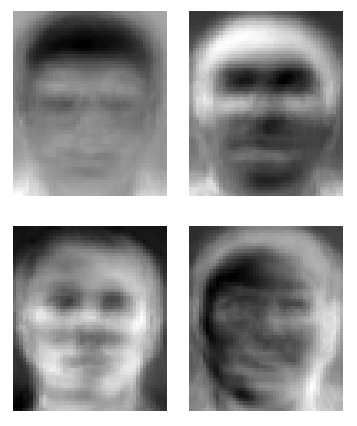
\includegraphics[width=0.7\textwidth]{../Files/eigenfaces.png}
    \caption{Example: Face detection result on a webcam image.}
    \label{fig:webcam-example}
\end{figure}

\begin{figure}[ht!]
    \centering
    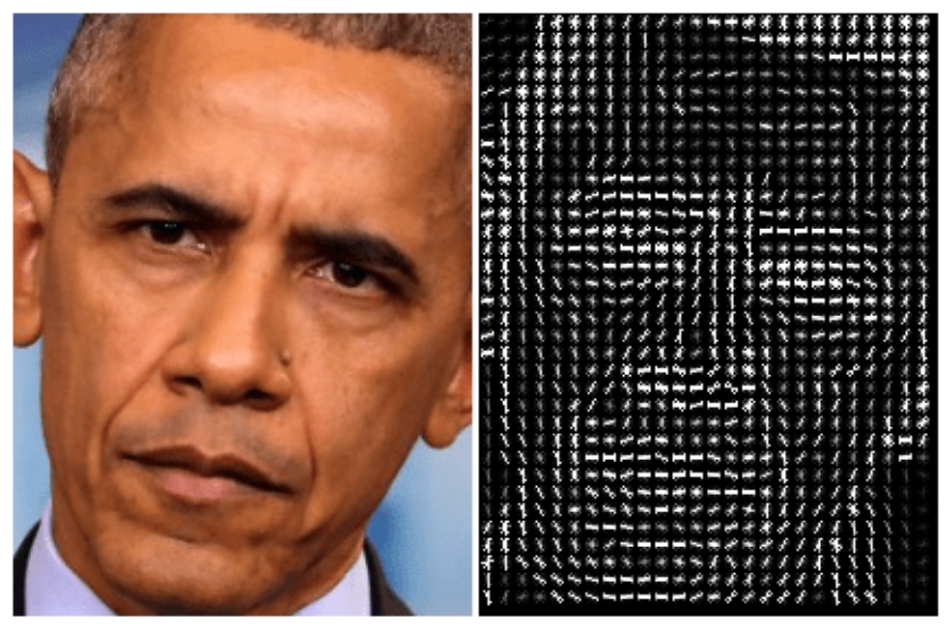
\includegraphics[width=0.7\textwidth]{../Files/histagram_of_oriented_gradients.png}
    \caption{Example: Face detection result on a security camera image.}
    \label{fig:seccam-example}
\end{figure}

\begin{figure}[ht!]
    \centering
    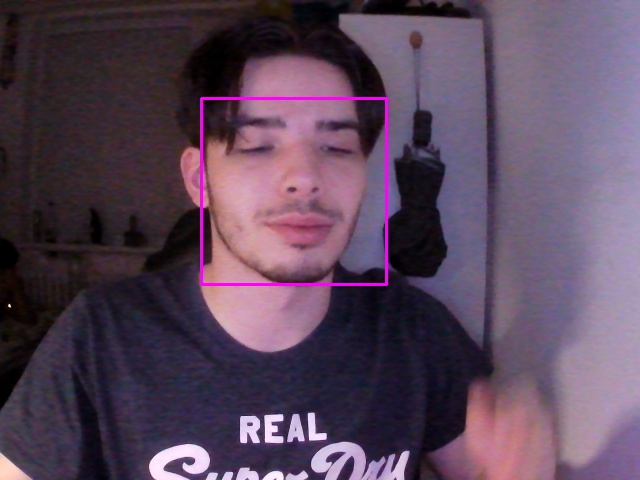
\includegraphics[width=0.7\textwidth]{../Files/webcam_result.jpg}
    \caption{Detected faces on webcam input.}
    \label{fig:webcam-result}
\end{figure}

\begin{figure}[ht!]
    \centering
    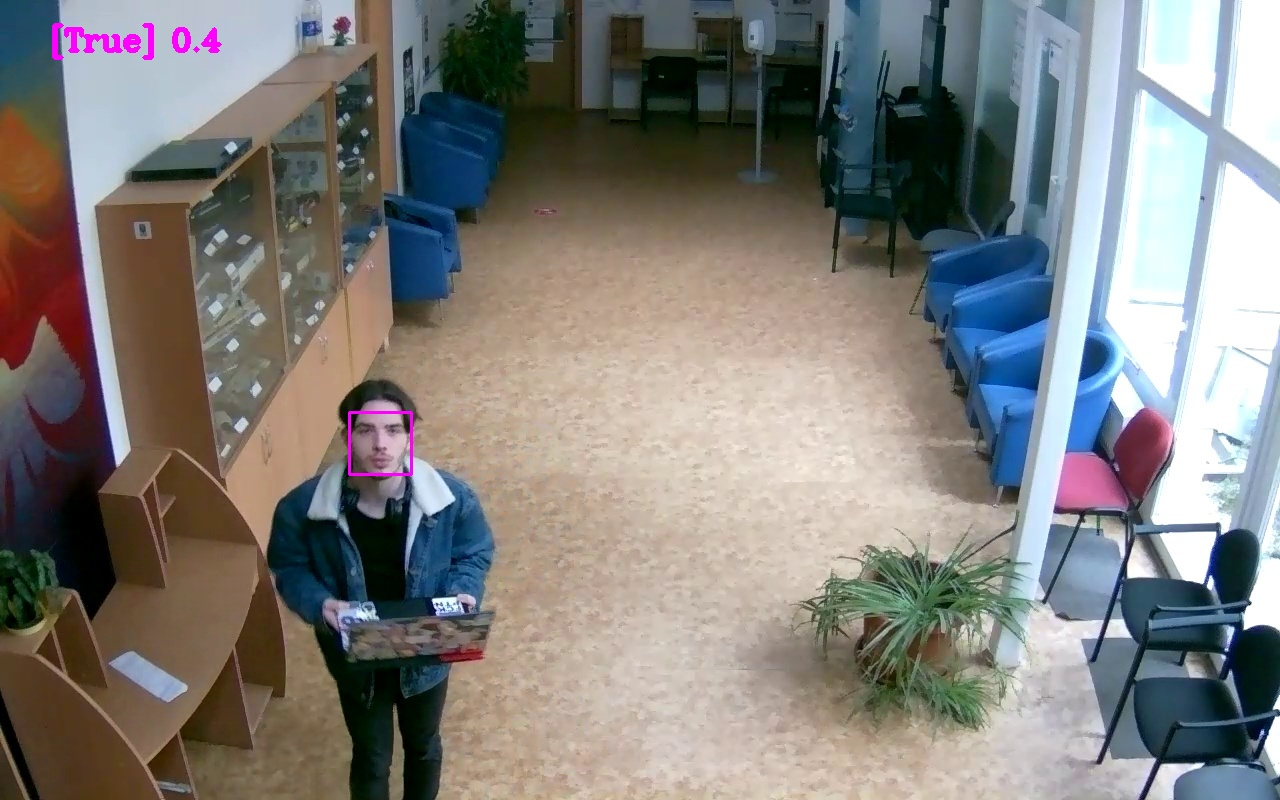
\includegraphics[width=0.7\textwidth]{../Files/seccam_result.jpg}
    \caption{Detected faces on security camera input.}
    \label{fig:seccam-result}
\end{figure}

% Attachments: CD, User Manual, System Manual

\subsection*{CD Attachment}
A CD containing the full thesis, codebase, datasets, and supplementary materials is attached as Appendix D.

\subsection*{User Manual}
The user manual for the face recognition attendance system is provided as Appendix E.

\subsection*{System Manual}
The system manual, including installation and deployment instructions, is provided as Appendix F.

% Add more figures/tables as needed.
\section*{Appendix B: Code Samples}
\addcontentsline{toc}{section}{Appendix B: Code Samples}

% Example code sample for face detection (OpenCV)
\begin{verbatim}
# Example Python code for face detection
import cv2
face_cascade = cv2.CascadeClassifier('haarcascade_frontalface_default.xml')
img = cv2.imread('test.jpg')
gray = cv2.cvtColor(img, cv2.COLOR_BGR2GRAY)
faces = face_cascade.detectMultiScale(gray, 1.3, 5)
for (x, y, w, h) in faces:
    cv2.rectangle(img, (x, y), (x+w, y+h), (255, 0, 0), 2)
cv2.imshow('img', img)
cv2.waitKey(0)
cv2.destroyAllWindows()
\end{verbatim}

% Example code sample for dataset splitting
\begin{verbatim}
# Example Python code for splitting dataset into train/val/test
import os, numpy as np
all_images = os.listdir('images')
np.random.shuffle(all_images)
train_count = int(len(all_images) * 0.7)
test_count = int(np.ceil(len(all_images) * 0.15))
val_count = len(all_images) - train_count - test_count
train_files = all_images[:train_count]
test_files = all_images[train_count:train_count+test_count]
val_files = all_images[train_count+test_count:]
# Move files to appropriate folders as needed
\end{verbatim}

% Example citation of code in thesis:
% See Appendix~\ref{appendixb} for code samples used in the implementation~\cite{opencv_library, numpy_library}.

% Add more code samples as needed, referencing them in the main text.
\section*{Appendix C: Dataset}
\addcontentsline{toc}{section}{Appendix C: Dataset}

The dataset used for face recognition experiments consists of images collected from webcams and security cameras. The dataset is organized as follows:
\begin{itemize}
    \item \textbf{Images:} Stored in separate folders for each subset (train, validation, test).
    \item \textbf{Labels:} Annotated using the \texttt{labelme} tool, with bounding boxes or landmarks in JSON format.
    \item \textbf{Augmentation:} Additional images generated using Albumentations for improved robustness.
\end{itemize}

% Example statistics (replace with actual numbers if available):
\begin{itemize}
    \item Total images: \textit{N}
    \item Training set: \textit{N1} images
    \item Validation set: \textit{N2} images
    \item Test set: \textit{N3} images
\end{itemize}

\subsection*{Abbreviations and Terms}
\begin{description}
    \item[FRS] Facial Recognition Software
    \item[AI] Artificial Intelligence
    \item[IoU] Intersection over Union
    \item[CSV] Comma-Separated Values
    \item[JSON] JavaScript Object Notation
    \item[RTSP] Real Time Streaming Protocol
    \item[CD] Compact Disc
    \item[GUI] Graphical User Interface
    \item[API] Application Programming Interface
    \item[GPU] Graphics Processing Unit
    \item[CPU] Central Processing Unit
    \item[GDPR] General Data Protection Regulation
    \item[CCPA] California Consumer Privacy Act
    \item[CPRA] California Privacy Rights Act
\end{description}

% Add more abbreviations as needed.


% If User Manual and System Manual are provided as separate appendices, add:
% \include{appendixd} % CD
% \include{appendixe} % User Manual
% \include{appendixf} % System Manual
%
\section*{Appendix A: Additional Figures and Tables}
\addcontentsline{toc}{section}{Appendix A: Additional Figures and Tables}

% List of additional figures and tables referenced in the thesis

\begin{figure}[ht!]
    \centering
    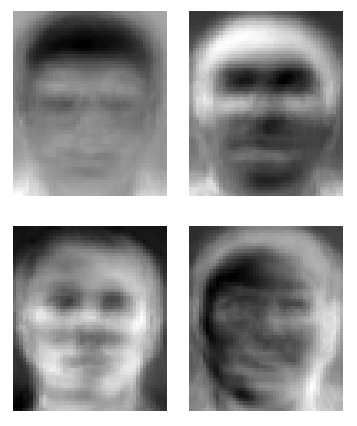
\includegraphics[width=0.7\textwidth]{../Files/eigenfaces.png}
    \caption{Example: Face detection result on a webcam image.}
    \label{fig:webcam-example}
\end{figure}

\begin{figure}[ht!]
    \centering
    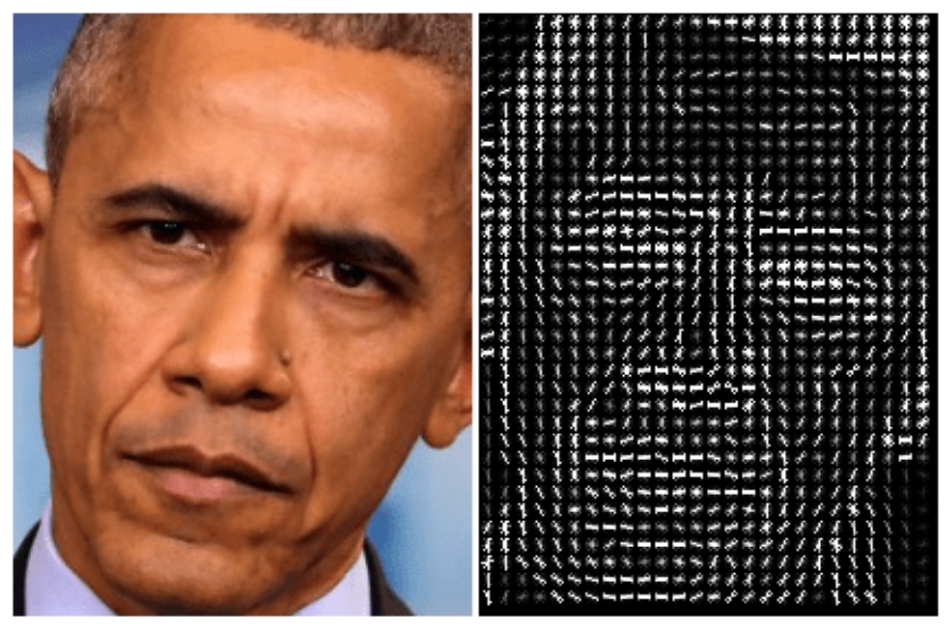
\includegraphics[width=0.7\textwidth]{../Files/histagram_of_oriented_gradients.png}
    \caption{Example: Face detection result on a security camera image.}
    \label{fig:seccam-example}
\end{figure}

\begin{figure}[ht!]
    \centering
    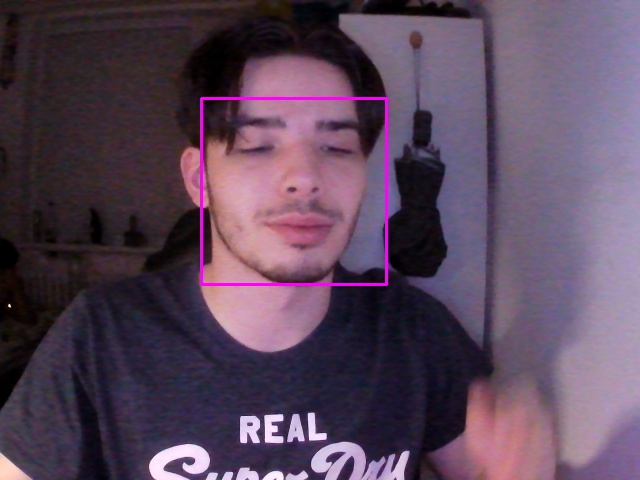
\includegraphics[width=0.7\textwidth]{../Files/webcam_result.jpg}
    \caption{Detected faces on webcam input.}
    \label{fig:webcam-result}
\end{figure}

\begin{figure}[ht!]
    \centering
    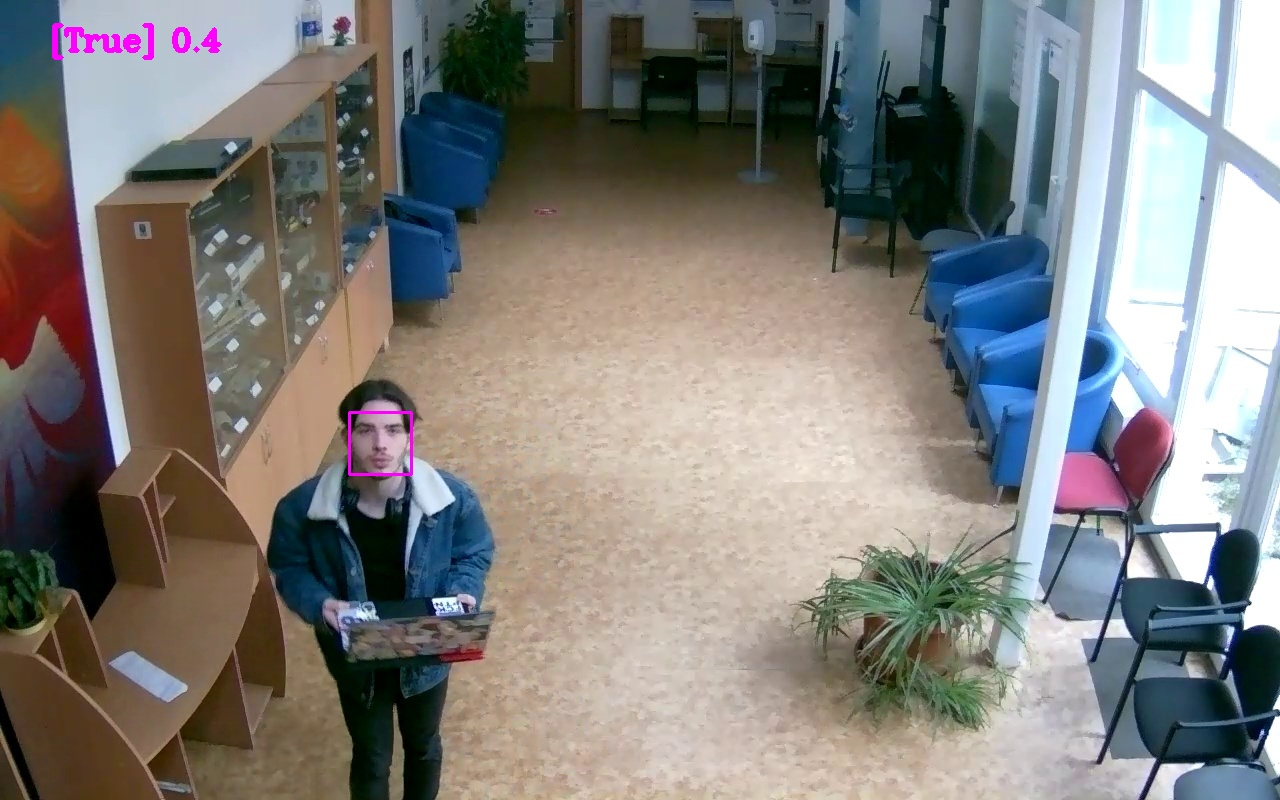
\includegraphics[width=0.7\textwidth]{../Files/seccam_result.jpg}
    \caption{Detected faces on security camera input.}
    \label{fig:seccam-result}
\end{figure}

% Attachments: CD, User Manual, System Manual

\subsection*{CD Attachment}
A CD containing the full thesis, codebase, datasets, and supplementary materials is attached as Appendix D.

\subsection*{User Manual}
The user manual for the face recognition attendance system is provided as Appendix E.

\subsection*{System Manual}
The system manual, including installation and deployment instructions, is provided as Appendix F.

% Add more figures/tables as needed. % CD
%
\section*{Appendix B: Code Samples}
\addcontentsline{toc}{section}{Appendix B: Code Samples}

% Example code sample for face detection (OpenCV)
\begin{verbatim}
# Example Python code for face detection
import cv2
face_cascade = cv2.CascadeClassifier('haarcascade_frontalface_default.xml')
img = cv2.imread('test.jpg')
gray = cv2.cvtColor(img, cv2.COLOR_BGR2GRAY)
faces = face_cascade.detectMultiScale(gray, 1.3, 5)
for (x, y, w, h) in faces:
    cv2.rectangle(img, (x, y), (x+w, y+h), (255, 0, 0), 2)
cv2.imshow('img', img)
cv2.waitKey(0)
cv2.destroyAllWindows()
\end{verbatim}

% Example code sample for dataset splitting
\begin{verbatim}
# Example Python code for splitting dataset into train/val/test
import os, numpy as np
all_images = os.listdir('images')
np.random.shuffle(all_images)
train_count = int(len(all_images) * 0.7)
test_count = int(np.ceil(len(all_images) * 0.15))
val_count = len(all_images) - train_count - test_count
train_files = all_images[:train_count]
test_files = all_images[train_count:train_count+test_count]
val_files = all_images[train_count+test_count:]
# Move files to appropriate folders as needed
\end{verbatim}

% Example citation of code in thesis:
% See Appendix~\ref{appendixb} for code samples used in the implementation~\cite{opencv_library, numpy_library}.

% Add more code samples as needed, referencing them in the main text. % User
%
\section*{Appendix C: Dataset}
\addcontentsline{toc}{section}{Appendix C: Dataset}

The dataset used for face recognition experiments consists of images collected from webcams and security cameras. The dataset is organized as follows:
\begin{itemize}
    \item \textbf{Images:} Stored in separate folders for each subset (train, validation, test).
    \item \textbf{Labels:} Annotated using the \texttt{labelme} tool, with bounding boxes or landmarks in JSON format.
    \item \textbf{Augmentation:} Additional images generated using Albumentations for improved robustness.
\end{itemize}

% Example statistics (replace with actual numbers if available):
\begin{itemize}
    \item Total images: \textit{N}
    \item Training set: \textit{N1} images
    \item Validation set: \textit{N2} images
    \item Test set: \textit{N3} images
\end{itemize}

\subsection*{Abbreviations and Terms}
\begin{description}
    \item[FRS] Facial Recognition Software
    \item[AI] Artificial Intelligence
    \item[IoU] Intersection over Union
    \item[CSV] Comma-Separated Values
    \item[JSON] JavaScript Object Notation
    \item[RTSP] Real Time Streaming Protocol
    \item[CD] Compact Disc
    \item[GUI] Graphical User Interface
    \item[API] Application Programming Interface
    \item[GPU] Graphics Processing Unit
    \item[CPU] Central Processing Unit
    \item[GDPR] General Data Protection Regulation
    \item[CCPA] California Consumer Privacy Act
    \item[CPRA] California Privacy Rights Act
\end{description}

% Add more abbreviations as needed.
 % System
\bibliographystyle{plain}
\bibliography{bib1}
\end{document}

%%
